\documentclass[../main/thesis_msc.tex]{subfiles}
\externaldocument{../appendex1.tex}
\begin{document}

\chapter{Scientific analysis}
In the course of this chapter, the results from the images obtained from the LOFAR data are explained. 
\section{Spectral index mapping}
\paragraph{Overview of method used:} Spectral index mapping involves several steps. One may use the task \verb|COMB| in \verb|AIPS|\footnote{\url{http://www.aips.nrao.edu/cgi-bin/ZXHLP2.PL?COMB}} or the task \verb|immath| in  \verb|CASA|\footnote{\url{https://casa.nrao.edu/docs/taskref/immath-task.html}}. However, it is not possible to obtain a satisfactory error distribution map using these methods. Hence, I obtained the spectral index map and the error map using the method described in this section. \\

\noindent The maps being used to obtain spectral index are of different frequencies, and hence have different inherent beam sizes. Hence, the map with higher spatial resolution is re-sampled to the resolution (lower) of the other map. This is generally done using the \textbf{convolution} operation. The Full Width at Half Maximum (FWHM) for both the synthesized beams values are converted to standard deviation using the formula valid for Gaussian distributions (Equation \ref{gaussian}).  

\begin{equation}
\sigma=\frac{\mathrm{FWHM}}{2\sqrt{2\textrm{ln}2}}.
\label{gaussian}
\end{equation}

The synthesized beams for the images that have been used in my case are circular. Equation \ref{convolution} shows the convolution formula used. $\sigma_{\textrm{New kernel}}$ is the standard deviation for the new Gaussian kernel that is to be used for convolving the higher resolution image. $\sigma_{\textrm{Higher frequency}}$ is the standard deviation of the synthesized beam of higher frequency image. $\sigma_{\textrm{LOFAR frequency}}$ is the standard deviation of synthesized beam for the LOFAR image. 

\begin{equation}
\sigma_{\textrm{New kernel}}=\sqrt{\left(\sigma_{\textrm{LOFAR frequency}}^2 - \sigma_{\textrm{Higher frequency}}^2\right)}
\label{convolution}
\end{equation}

The beam size is converted to pixel units by multiplying it with the pixel scale in the image. Once the size of the convolution kernel is known in pixel units, we Gaussian smooth (convolve) the higher resolution image to have the resolution of the lower resolution image. The images are usually of different sizes, and hence, to ensure that both the images are of the same size, bi-linear interpolation method using the `resize' function in sci-kit library of python can be used. Spectral index is calculated using the assumption that the intensity, I $\sim \nu^{-\alpha}$. The error maps are estimated using standard Gaussian error propagation. 

\subsection{IC\,342}
For IC\,342, the spectral index map is made using the images at 1.49~GHz frequency \citep{2015A&A...578A..93B} and the LOFAR map (at 145~MHz), as shown in Figure \ref{ic342_spectr}. The UV data from the VLA map uses the baselines from 200~$\lambda$ to 5200~$\lambda$. Though the LOFAR visibilities also have several short baselines due to the dense core, the shorter baselines need to be clipped so that both the maps are sensitive to the same angular scales. The images thus obtained are gridded to have the same grid using the \verb|AIPS| task \verb|OHGEO|. The LOFAR map is calibrated using the flux density scale as described in \citet{2012MNRAS.423L..30S}, while the VLA map was calibrated using the flux density scale as described in \citet{2017ApJS..230....7P}. The spectral index map is then computed pixel by pixel. The maps presented in this paper are made using a five-sigma filter on the noise levels for both the input images. Both the maps from the two frequencies have a resolution of 45~arcsec. The images of this resolution have been used because the higher resolution images from the LOFAR map still contain several artifacts, while the 45~arcsec image can be seen to have better depiction of diffuse emission. \\

We plot the histogram showing the distribution of spectral indices values from the Figure \ref{ic342_spectr} in the Figure \ref{icsp}, and find that the median value is -0.52 for IC\,342. The binning has been done using the Freedman-Diaconis rule\footnote{According to this rule, the bin size, B = 2 $\times \frac{\textrm{IQR(x)}}{\sqrt[3]{\textrm{n}}}$, where IQR(x) is the interquartile range, and n is the number of observations in the sample $x$.}\\
\begin{figure}
  \centering
  \begin{tabular}{@{}c@{}}
    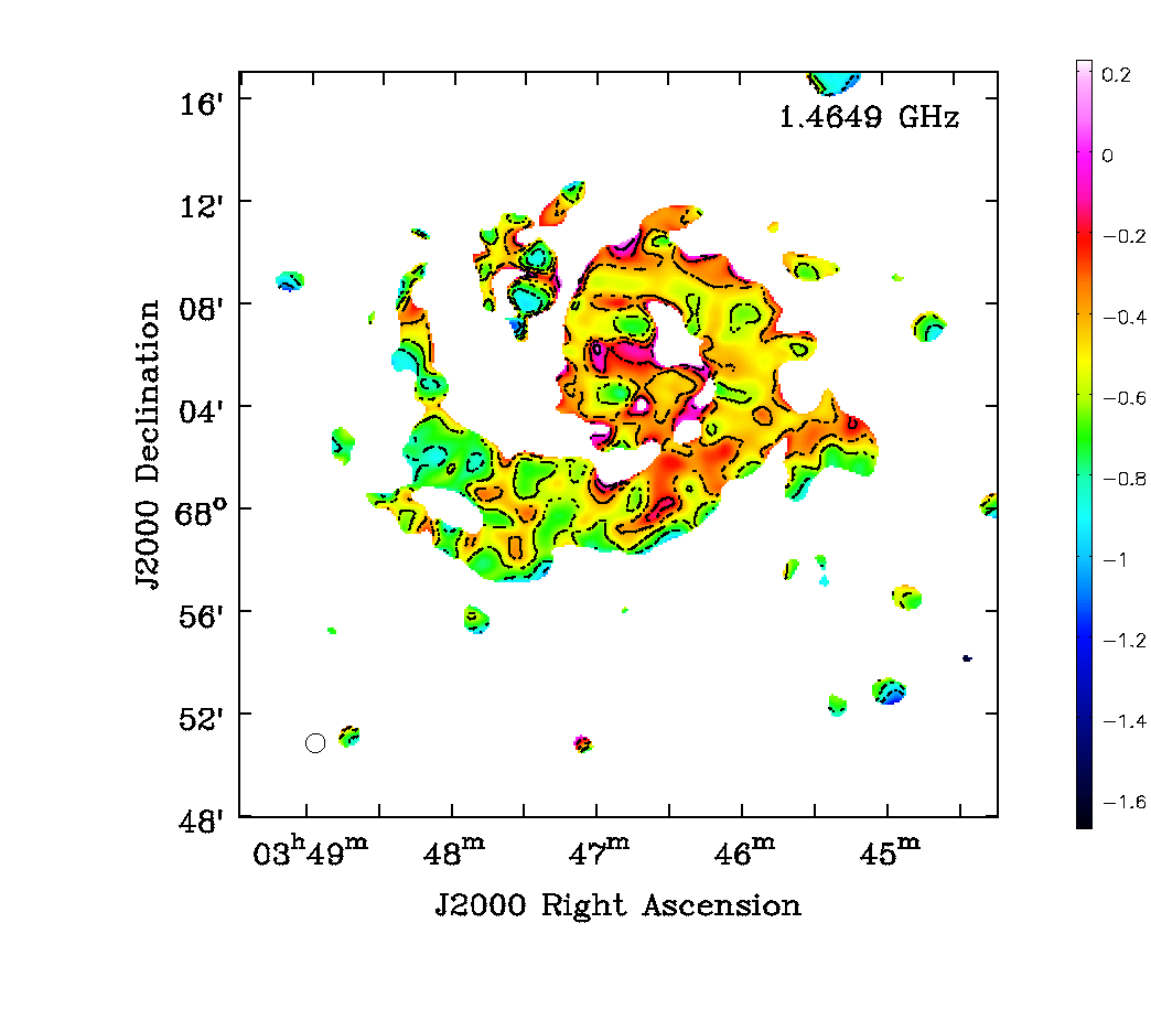
\includegraphics[scale=0.25]{13ic_Spectral.png} \\[\abovecaptionskip]
    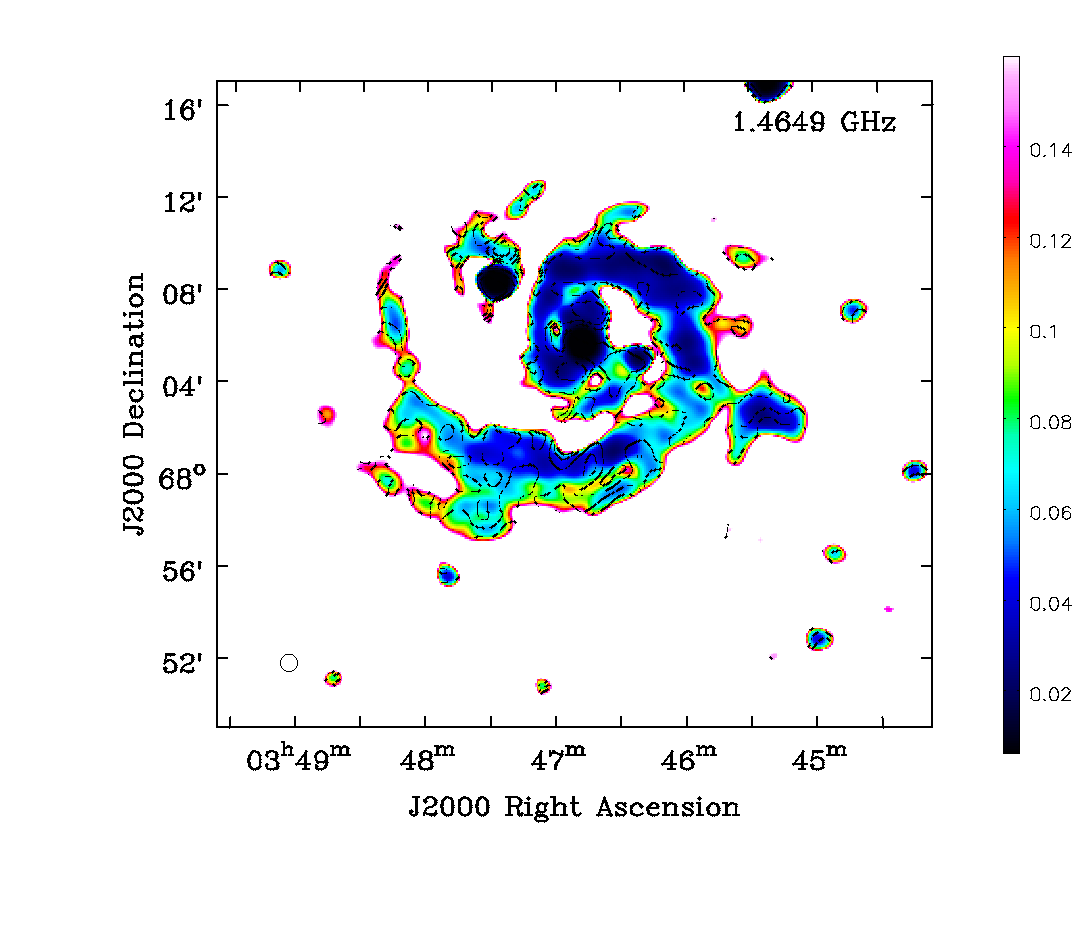
\includegraphics[scale=0.35]{13Spectral_error_ic.png} \\[\abovecaptionskip]
  \end{tabular}
  \caption{\textit{Above:} The spectral index map of IC\,342 obtained from 1.4~GHz VLA map and 145~MHz LOFAR map at 45" resolution. It uses values above 5$\times$ the noise level (5$\sigma$) from the VLA and LOFAR maps. The contours on the map are 0.2, 0.4, 0.6, 0.8, 1, 0 $\times$ -1. \textit{Below:} The error map for the spectral index map. The contours are the same  for both the images.}
	\label{ic342_spectr}
\end{figure}

\begin{figure}
\centering
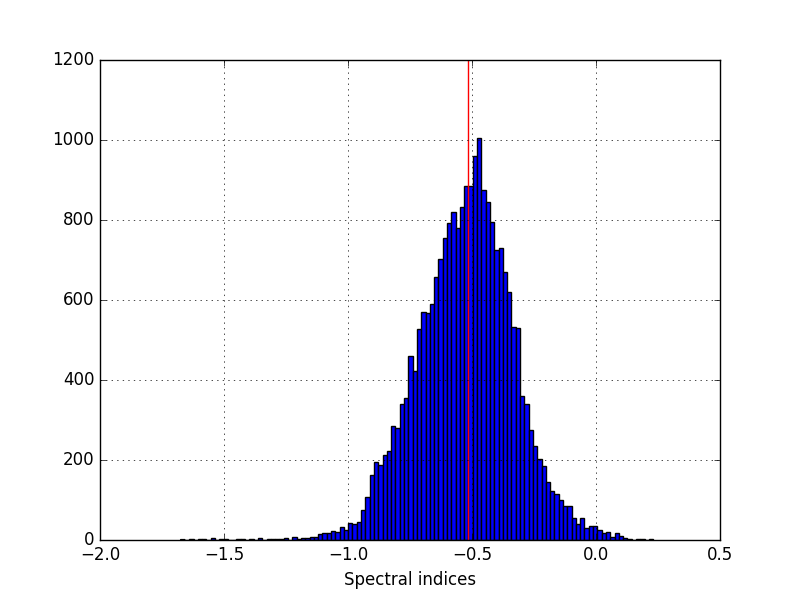
\includegraphics[scale = 0.5]{spectral__histogram_cumu_ic.png}
\caption{The spectral index distribution for IC\,342 for the spectral index map shown in Figire \ref{ic342_spectr}. The binning is done according to  Freedman-Diaconis Rule \citep{Freedman1981}}
\label{icsp}
\end{figure}

\subsection{NGC\,628}
For NGC\,628, the spectral index maps depicted in Figure \ref{ngc_spectr}, have been made using the maps from frequency 3~GHz using VLA data and 141~MHz LOFAR map. Due to the absence of UV calibrated data, we convolve both LOFAR and VLA maps to have the same resolution of 20~arcsec. The images are then regridded using \verb|OHGEO| task in \verb|AIPS| and the spectral index map is made with 3-sigma flux densities (3 times the noise level in the individual maps) for both the images. The 20~arcsec image was chose for the LOFAR map because it has a higher Signal to Noise ratio than the other images, while curbing the artifacts. The VLA image used had a resolution of 18~arcsec, and is convolved to have a resolution of 20~arcsec. \\

In the Figure \ref{ngcsi}, one can take a look at the histogram showing the distribution of spectral index values from the Figure \ref{ngc_spectr}. The median value for the spectral index values is -0.86, which is the steepness expected from synchrotron emission.

\begin{figure}
	\centering
    \begin{tabular}{@{}c@{}}
	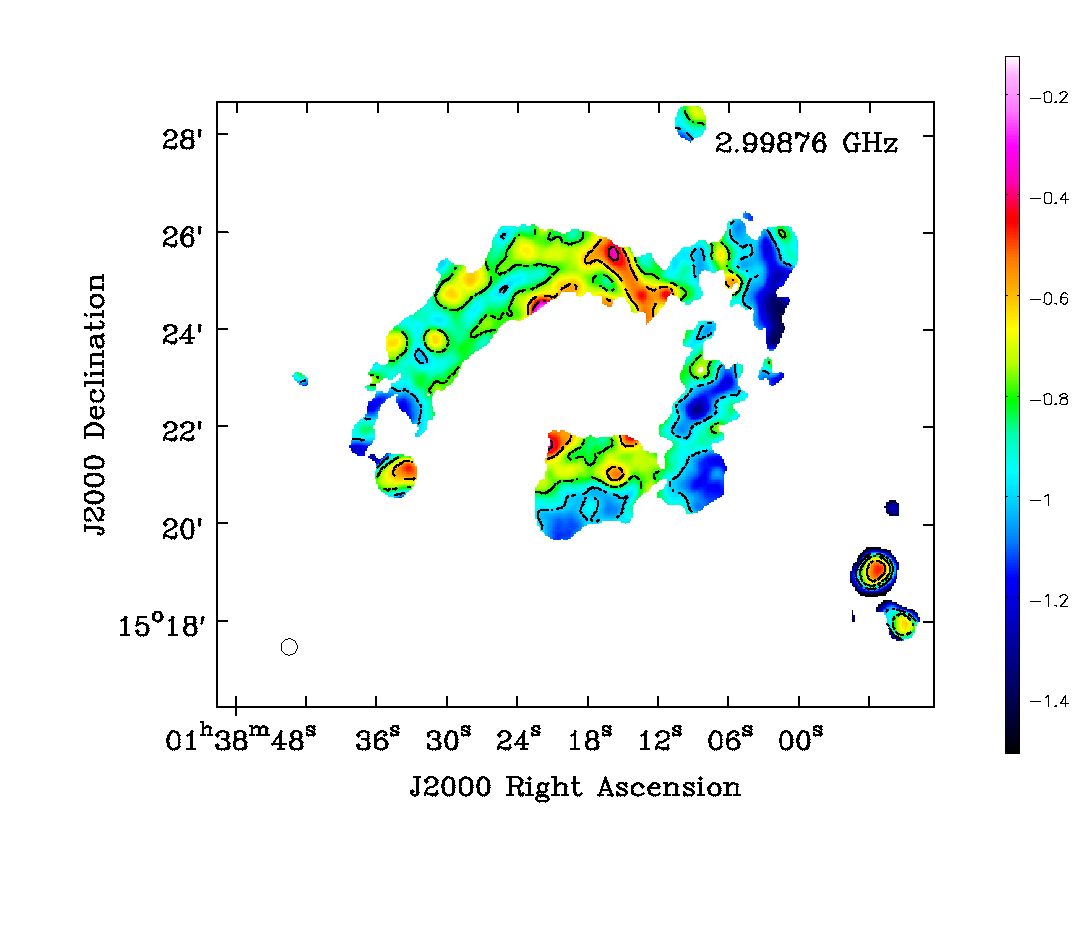
\includegraphics[scale = 0.45]{ngc_3sig_13.png} \\[\abovecaptionskip]
	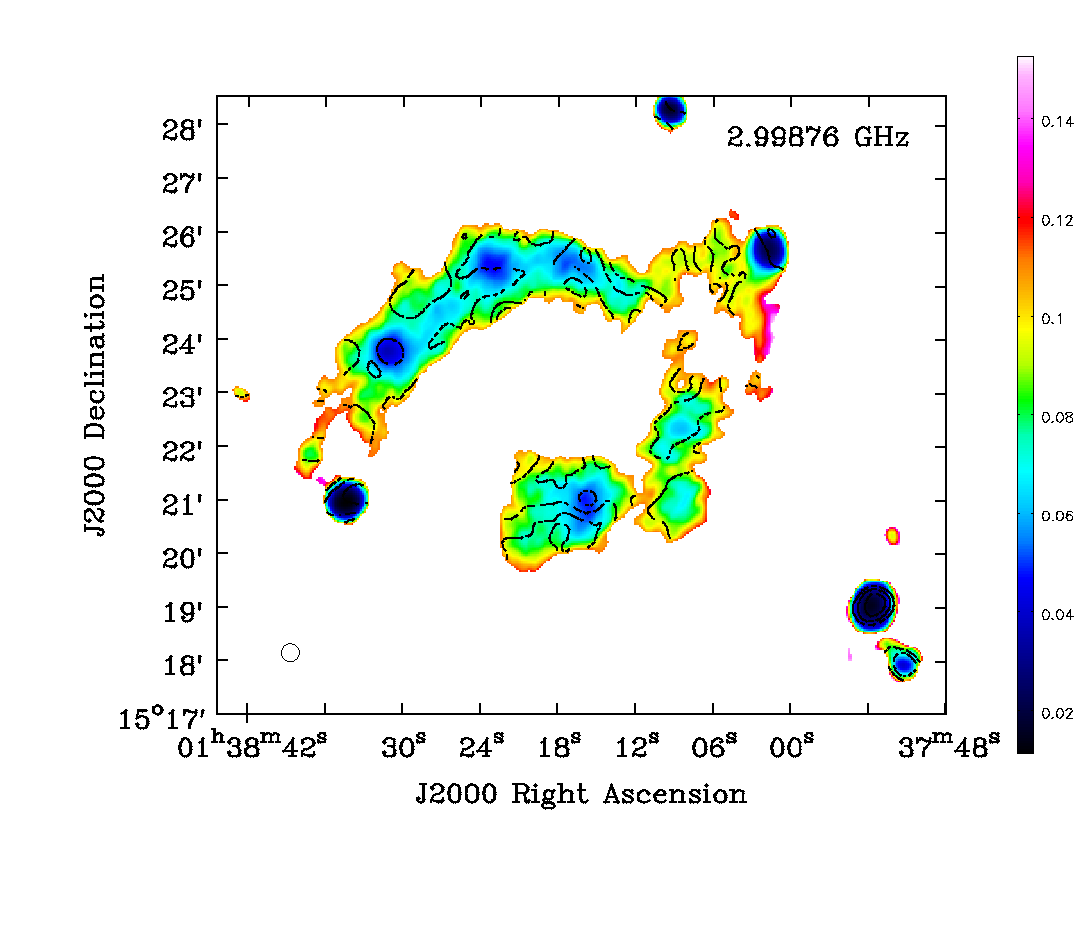
\includegraphics[scale = 0.45]{ngc_3sig_13_err.png}\\[\abovecaptionskip]
	\end{tabular}
	\caption{\textit{Above:} The spectral index map for NGC\,628 obtained from 3~GHz VLA map and 145~MHz LOFAR map at 20" resolution. This is a 3-sigma spectral index map. The contours on the map are 0.2, 0.4, 0.6, 0.8, 1, 0 with unit contour level of -1. \textit{Below:} The error map for the spectral index map. The contours are the same for both the images.}
	\label{ngc_spectr}
\end{figure}

\begin{figure}
\centering
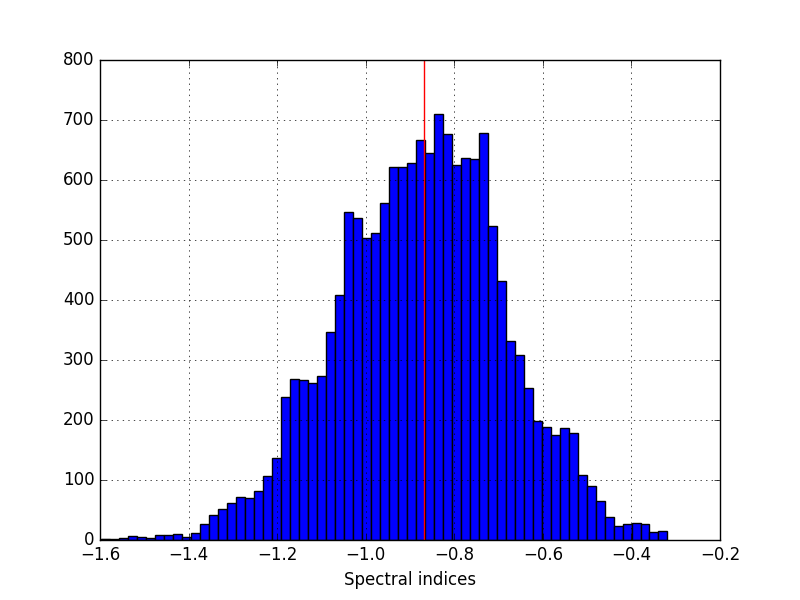
\includegraphics[scale = 0.45]{spectral__histogram_cumu.png}
\caption{This histogram shows the distribution of the spectral index values for NGC\,628. The median lies at -0.86 (expected value).}
\label{ngcsi}
\end{figure}

\section{Interpretation of spectral index maps}

One can learn about the process involved in the galaxy with the help of spectral index maps. The Figure \ref{therm} shows various process involved in a galaxy at low radio frequencies that influence the spectrum can be seen. The spectral index for synchrotron emission is -0.7 and that of thermal emission is -0.1. Thermal absorption is a process that is important especially in star forming galaxies, and explains the flat spectrum when very low frequencies are considered. If one considers the spectral index values between frequencies $\nu_2$ and $\nu_3$, a flat spectral index is seen. This flatness is because of the thermal emission at the $\nu_3$ frequency. If one considered the spectral index between frequencies $\nu_1$ and $\nu_2$, the flat spectral index is explained by thermal absorption.

\begin{figure}
\centering
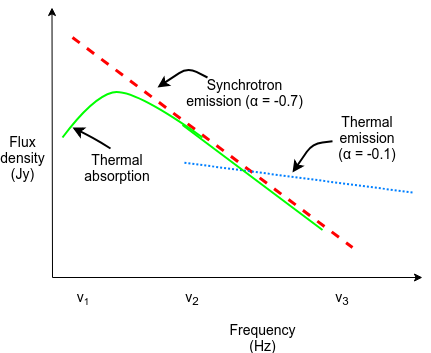
\includegraphics[scale = 0.5]{SED_corr.png}
\caption{Spectral Energy Distribution (SED) for the three process important in star forming galaxies like IC\,342. The red dashed line indicates synchrotron emission, and has a spectral index value ($\alpha$) of -0.7. The thermal emission is indicated by the blue dotted line, and has a spectral index value of -0.1. Thermal absorption process is indicated by the green curve. This process is responsible for the flattening of the spectral index at low radio frequencies. Based on the two frequencies considered to obtain the spectral index, the flattening and steepening of the spectrum can be explained.}
\label{therm}
\end{figure}

\subsection{IC\,342}
The Figure \ref{ic342_spectr} shows the spectral index map obtained for IC\,342. The edges and the inter-arm regions of IC\,342 can be seen to have a steep spectral index. This means that the flux density for the galaxy in the VLA map is much lower than that of the LOFAR map. This implies the presence of a higher level of the synchrotron emission that is traced at lower frequencies. A steep spectral index indicates the presence of low energy, older electrons that have traveled farther away from the spiral arms and the central region where the star formation occurs. Hence, the steep spectral index is expected at these regions.\\


Flatter spectral index (0.2 to -0.2) can be seen in the center of the galaxy. Flat spectral indices imply that the flux density values for VLA and the LOFAR maps have only a small difference. With the help of the Spectral Energy Distribution (SED), it can be argued that the flat spectral index can happen because of either an increase in the flux density of the galaxy in the VLA map because of thermal emission, or from a decrease in the flux density of the galaxy in LOFAR map because of thermal absorption. 

\paragraph{Thermal emission:} To examine which process results in the flat spectral index in my case, we first try to obtain the thermal fractions required to explain such a flat spectral index. The thermal and non-thermal components are separated by assuming a constant spectral index ($\alpha_{\textrm{nth}}$) of $-$0.7 and $-$0.5 for synchrotron emission, and a thermal spectral index ($\alpha_{\textrm{th}}$) of $-$0.1 for thermal emission. The resulting thermal fractions ($f_{\textrm{th}}$) are listed in Table \ref{allph}. These fractions seem too high for a galaxy. \citet{2015A&A...578A..93B} found that the thermal fraction at $\lambda$6.2~cm is about 50\% in the central region and 20\% to 30\% in the spiral arms and 10\% or less in the inter-arm region\footnote{Although it was argued that the thermal fraction is overestimated in the spiral arms because of their method used.} at 1.49~GHz.\\

\begin{table}
\centering         
        \begin{tabular}{cccccc}
        \hline\hline  
             $\alpha_{\textrm{obs}}$ & $f_{\textrm{th}_{-0.7}}$ (145~MHz) & $f_{\textrm{th}_{-0.7}}$ (1490 MHz) & $f_{\textrm{th}_{-0.5}}$ (145 MHz) & $f_{\textrm{th}_{-0.5}}$ (1490 MHz)\\
            \hline
            $-$0.7 & 0\% & 0\% &-&-\\
			$-$0.6 & 9\% & 28\% &-&-\\
			$-$0.5 & 19\% & 49\% &0\% & 0\%\\
			$-$0.4 & 33\% & 67\% & 17\% & 34\%\\
			$-$0.3 & 51\% & 81\% & 39\% &61\%\\
			$-$0.2 & 72\% & 91\% & 66\% & 83\%\\
			$-$0.15 & 85\% & 96\%& 82\% & 92\%  \\
			$-$0.1 & 100\% & 100\% & 100\%& 100\%\\
            \hline
        \end{tabular}
\caption{If a spectral index for synchrotron emission is assumed as $-$0.7 and thermal emission is assumed as $-$0.1, the percentage of thermal fraction for the observed spectral index values (between frequencies of 145 to 1490~MHz, $\alpha_{\textrm{obs}}$) are obtaind ( represented as $f_{\textrm{th}_{-0.7}}$), at the two frequencies --- 145~MHz and 1.49~GHz. The same is done when the spectral index for synchrotron emission is assumed to be $-$0.5 and the thermal fraction is represented as $f_{\textrm{th}_{-0.7}}$ These values have been obtained using the code from Dr. Beck (priv. comm).}
\label{allph}  
\end{table}

\citet{2017ApJ...836..185T} found that the thermal fractions in galaxies is around 10\%. If one uses this value to be the thermal fraction in IC\,342, then for the observed spectral index values of $-$0.4, $-$0.3, $-$0.2 and $-$0.15, one must assume that the synchrotron spectral index value is $-$0.63, $-$0.53, $-$0.42, $-$0.32, $-$0.21 and $-$0.16 respectively. This shows that for these spectral indices, thermal emission does not satisfactorily explain the observed flat spectral indices, as it is not physically valid according to existing models of cosmic ray electron accelaration. \\

\paragraph{Thermal absorption:} In order to see if the flat spectral index values are because of free-free absorption, the thermal map obtained from 1.49~GHz is overlaid on the spectral index map. The thermal map traces the regions of star formation activity. Hence, the regions in which the thermal flux density is higher, there is a higher Star Formation Rate (SFR). These SF regions would result in \textbf{free-free absorption}, resulting in a decrease in the flux density of the galaxy at the lower frequency.  \\

From the Figure \ref{hlaph_ic}, we can see that the higher thermal flux density region coincides with the regions of flatter spectral index. Furthermore, from \citet{ic342_3}, we know that several dense (with electron densities of around 104-105 cm$^{-3}$), and compact ($\leq$0.1~pc) H II regions are predicted to exist in the nucleus of the galaxy. These regions are known to be heated by the ionizing photons from the early-type stars. They are cooled by lines excited from collisions such as C II line of wavelength 158~$\mu$m. Free-free absorption is especially pronounced in H\,II regions as explained in Chapter 1. So, we can conclude that the LOFAR synchrotron flux density in the nuclear region is decreased due to the presence of such H\,II regions, that give rise to free-free absorption. In the Figure \ref{swr}, we can take a look at the position of the H\,II regions existing in the nucleus of the galaxy. \\
\begin{figure}
\centering
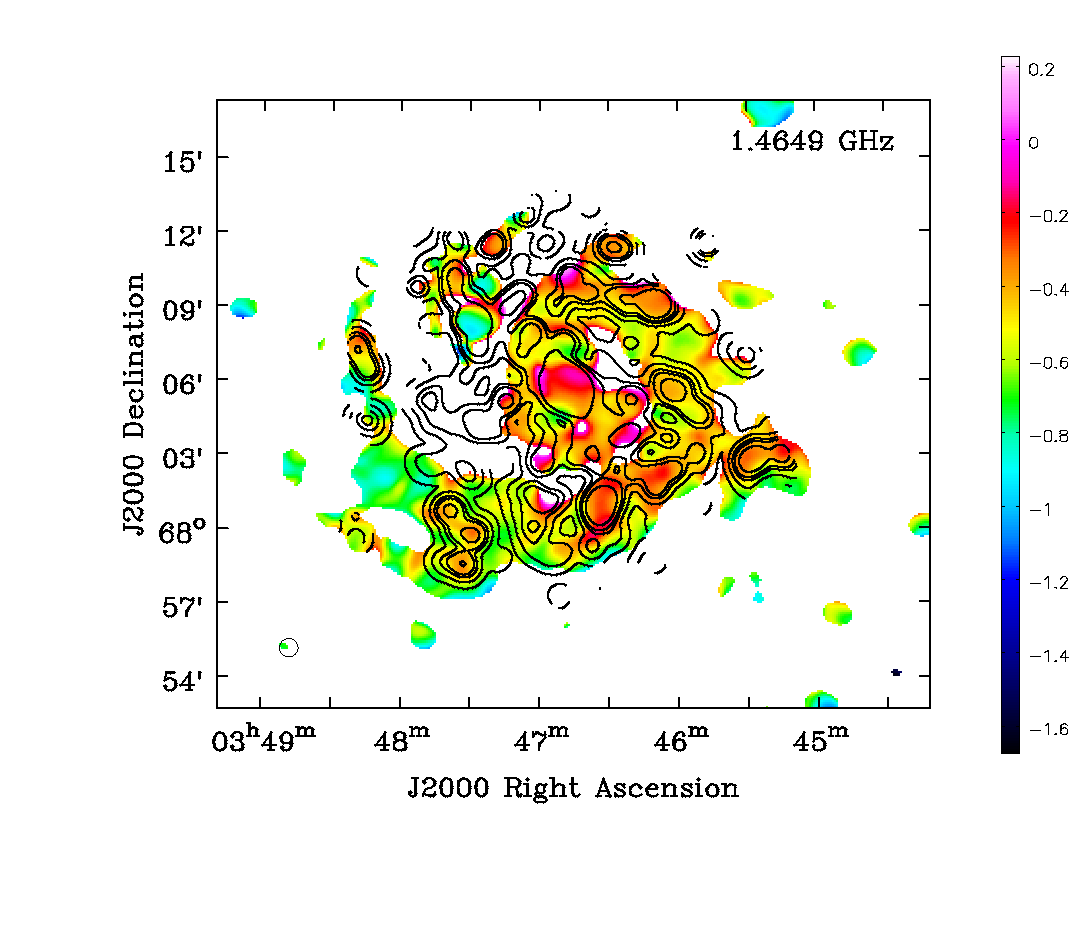
\includegraphics[scale = 0.435]{13_thermal_IC.png}
\caption{This image depicts the correlation of the flatter spectral index and the presence of thermal emission. The contours are 0.5, 5, 18, 32, 80 of the thermal map with unit contour level of 10~mJy/beam }
\label{hlaph_ic}
\end{figure}
In order to understand the correlation better, we plot the correlation between the flux densities of the thermal map with the spectral index values for each pixel. From the Figure \ref{corr_ic}, we can see that the pixels with a higher flux density of the thermal map, have a much flatter spectral index value. Thus, we can conclude that the free-free absorption regions with high star formation give rise to flat spectral index. \\
\begin{figure}
\centering
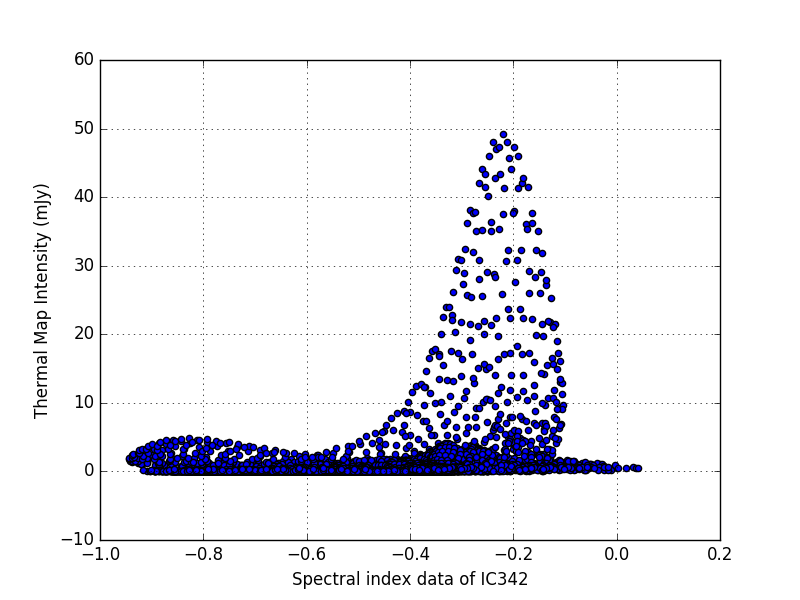
\includegraphics[scale = 0.5]{IC_corre.png}
\caption{Correlation of the thermal intensity values with the spectral index map values for IC\,342. The spectral index values are obtained by clipping the values of flux densities lower than 5$\times$ the noise level in 1.49~GHz and 145~MHz map, for each pixel. From the Figure, it is evident that regions with higher radio thermal flux density which indicate the presence of free-free absorption from star forming regions, have a flatter spectral index values. The 'tail' seen at the right hand portion showing the discrepency may be because of the missing diffuse flux density that affects spectral indices at low intensity.}
\label{corr_ic}
\end{figure}
I also plot a Far Infra Red (FIR) map of 350~nm over the galaxy, that is from the KINGFISH project (Key Insights on Nearby Galaxies: a Far-Infrared Survey with Herschel) \citep{2011PASP..123.1347K}. FIR emission comes from re-radiation by dust, which has been heated by ultra violet (UV) photons. These photons are emitted by massive and short-lived stars. The diffusion length of a CRE is much larger than the mean free path of an FIR photon, a radio continuum image would appear as a smoothed version of a FIR image. The Figure \ref{FIRic} shows the correlation of the star forming regions with that of flat spectral index, indicated by the redder regions.
\begin{figure}
\centering
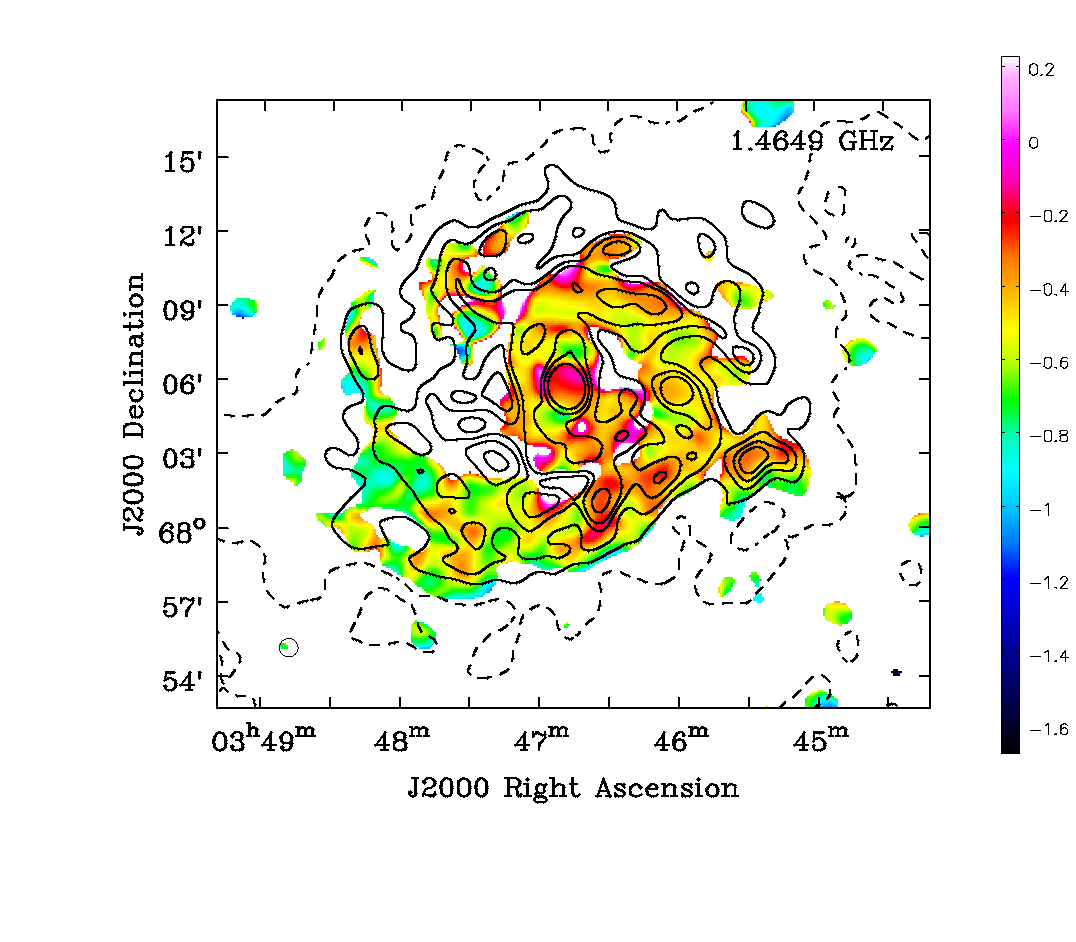
\includegraphics[scale = 0.5]{13_FIR_IC.png}
\caption{The overlaid plot is the FIR map of IC\,342 at 350$\mu$m. One can notice the correlation of flatter spectral index and higher flux density of this map. The contours represent 0.2, 0.4, 0.6, 0.8, 1, 1.5, 2, 3 $\times$ 15~Jy/beam.}
\label{FIRic}
\end{figure}

\subsection{Case of missing flux}
\noindent We plot the integrated flux density within successive radii of width 0.5~arcmin and obtain the plots shown in Figure \ref{ic342_ring}. This is done for both the 20~cm map and the LOFAR map, with full UV coverage for both the maps. We find that the total flux density integrated to 10', S$_{\textrm{LOF}}$ = 4.82$\pm$0.22~Jy for the LOFAR map. For the 20~cm map, this value is S$_{\textrm{VLA}}$ = 2.26$\pm0.13$~Jy. This shows that there is a lot of missing flux in the LOFAR map, if we consider the existence of only synchrotron emission.\\
In order to figure out the amount of missing flux, we first extrapolate the flux density values obtained for IC\,342 using the values found by \citet{2017ApJ...836..185T} at higher frequencies, and obtain the spectral index as -0.76. As can be seen from figure \ref{taba}, the $\alpha$ value is extrapolated to 145~MHz, we expected flux density value is obtained, S$_{\textrm{EXP}}$ = 10.7~Jy. \\


\begin{figure}[h]
\centering
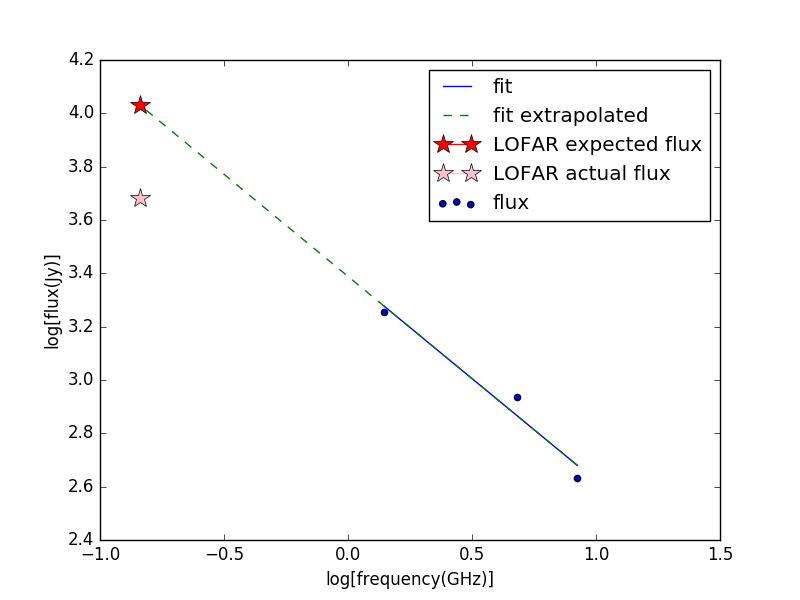
\includegraphics[scale = 0.5]{Taba_SED_values_IC342.png}
\caption{This plot shows the flux density values from previous study done for the galaxy by \citet{2017ApJ...836..185T} for IC\,342 as blue dots, with the fit shown in blue line. The green dashed line represents the extrapolated fit with the slope of -0.76. The pink star represents the flux density from the LOFAR map, and the red star represents the expected flux density for the frequency of 145~mHz.}
\label{taba}
\end{figure}

Thus, the amount of missing flux density, $\Delta$S = S$_{\textrm{EXP}} -$S$_{\textrm{LOF}} \approx$ 5.9~Jy. The missing flux density per unit beam is given by:
\begin{equation}
\frac{\Delta\textrm{S}}{\textrm{N}} = \Delta\textrm{S} \left(\frac{\textrm{Area of integration (in arcmin)} \times \textrm{cos}i}{1.13 \times \textrm{Resolution of image (in arcmin)}}\right) \approx 14~\textrm{mJy/beam},
\end{equation}
where $i$ is the angle of inclination. This value is almost 36 times the rms noise in the image. This means that a lot of the diffuse flux density is missing.\\

One explanation for the flux density to be low is thermal absorption. The inner part of IC\,342 has a high amount of thermal absorption as is seen from the flat spectral index at the center. Hence, we obtain the amount of missing flux density due to thermal absorption by obtaining the flux density value within 3' radius of the galaxy (with the galaxy's center as its center). This is done between maps that have the same UV baseline coverage with the rest of the baselines clipped, as the diffuse flux in both the maps would be missing, leading to a fair comparision between the two maps. \\

The amount of thermal absorption is obtained by extrapolating the flux density of the VLA map within 3' to obtain the expected flux density at the frequency of LOFAR, using the relation S $\propto \nu^{\alpha}$, with alpha being the spectral index (-0.5\footnote{This spectral index is taken as a combined $\alpha$ value for thermal emission and synchrotron emission.}). S$_{\text{3'}}$ is the flux density observed in the LOFAR map within the radius of 3'.
\begin{alignat}{2}
\frac{\textrm{S}_1}{\textrm{S}_2} 
&= \left(\frac{\nu_1}{\nu_2}\right)^{\alpha}\\
\textrm{S}_1
&= \textrm{S}_2 \left(\frac{\nu_1}{\nu_2}\right)^{-0.5}\\
\textrm{S}_1 & =273\text{~mJy} \left(\frac{145}{1490}\right)^{-0.5} \approx 870\text{~mJy}\\
\text{S}_{\text{3'}} 
&=555\text{~mJy} \\
\Rightarrow \text{Flux lost due to thermal absorption} 
& \approx 300 \text{~mJy}
\end{alignat}
With the help of this correction flux density value, we can figure out the amount of flux density missing in the overall galaxy (i.e., for the galaxy upto a radius of 10'). 
\begin{alignat}{2}
  \textrm{Correction} 
  &\approx 300\text{~mJy}\\
  \text{S}_{\textrm{EXP}}
  &=688\left(\frac{1.49}{0.145}\right)^{0.74}
  \approx 3.72\text{~Jy}&\\
  \text{S}_{\textrm{LOF}}
  &=\underbrace{1.4}_{\textbf{A}} + \underbrace{0.3}_{\textbf{B}} \text{~Jy}  \approx 1.7 \text{~Jy}& \label{lofex}\\
  \Rightarrow \Delta\text{S} &=3.72-1.7 \approx 2.02  \text{~Jy}\\
  \text{Missing flux/beam} &=\frac{\Delta\text{S}}{\text{N}}\approx 4.47\text{~mJy}&
\end{alignat}
where \textbf{A} and \textbf{B} in Equation \ref{lofex} represents the flux from my LOFAR map of the galaxy upto a radius of 10' and the thermal absorption flux density of the galaxy obtained respectively. If one considers the value of -0.5 as the value of the overall spectral index of the galaxy upto a radius of 10', then this value is reduced is \textbf{1.1~mJy}. This value of only 1.6 times the noise level.\\
\paragraph{Scale height:}The integrated flux density values for IC\,342 for successive radii in rings with a width of 0.5' (about 0.5~kpc) are obtained, with the center of the rings aligned at the center of the galaxy. The plot with the radial profile using the obtained values is shown in Figure \ref{ic342_ring}. This is done for the images of the two frequencies- 145~MHz and 1.49~GHz, with the maps made using the full UV range. We also obtain the scale lengths \footnote{The scale length is defined as the radius at which the flux density of the galaxy has fallen off by a factor of e (2.71828) from the center. The flux density can be written as the function: 
\begin{center}
I=I$_0$exp$\left(^-\frac{r}{r_0}\right)$
\end{center}
Here, I$_0$ is the flux density in the center of the galaxy and $r_0$ is the scale length. Hence, when plotting lnI as a function of the radius r, the scale length is given by r$_0$ = $-\frac{1}{\textrm{S}}$, where S is the slope of the fitted linear line}for the two maps. For the LOFAR map, it is 15~arcmin, which is around 14.8~kpc. The scale height for the 20~cm map, it is 19~arcmin, which is around 18.7~kpc. Scale length shows the distance traveled by the CRE that is giving out that frequency photon. Here, an electron emitting the photon in LOFAR frequency (145~MHz) travels a distance of 14.8~kpc. Due to the longer life-time of the cosmic ray electrons that are detected using the LOFAR map, we should be able to see a longer scale length in the case of LOFAR map. However, this is not the case, which shows that the LOFAR map has less diffuse flux from the extended emission than is expected.

\begin{figure}
	%\centering
	\subfloat[]{{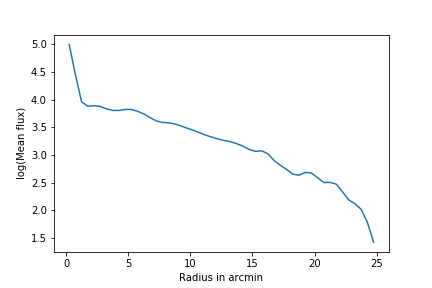
\includegraphics[scale = 0.5]{VLA_scale_length.png}}}
	\centering
	\subfloat[]{{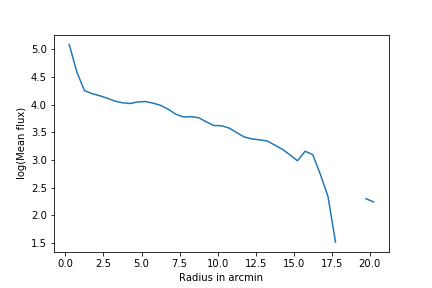
\includegraphics[scale = 0.5]{LOFAR_scale_length.png}}}
	\caption{The radial profiles for the full UV range maps. \textit{Left:} The radial profile of the galaxy IC\,342 i.e., radius vs log of integrated flux density for 20~cm map. \textit{Right:} The radial profile for the LOFAR map. The bright background source for both the images has been subtracted before the integration has been performed.}
	\label{ic342_ring}
	\end{figure}

\paragraph{Comparision with spectral index maps at other frequencies:}The Figure \ref{specic} shows the spectral index values obtained between $\lambda$6.2~cm and $\lambda$20.1~cm at 25" resolution \citep{2015A&A...578A..93B}. As the wavelengths of the two maps in Figure \ref{specic} are lower, the flatness in the spectral index can be explained by thermal emission (the flux density in this case is higher for the lower wavelength--- $\lambda$6.2~cm map, resulting in a flat spectrum). The spectral index in the inter-arm regions and in the outer disk is steep, as expected, due to synchrotron emission.

\begin{figure}
\centering
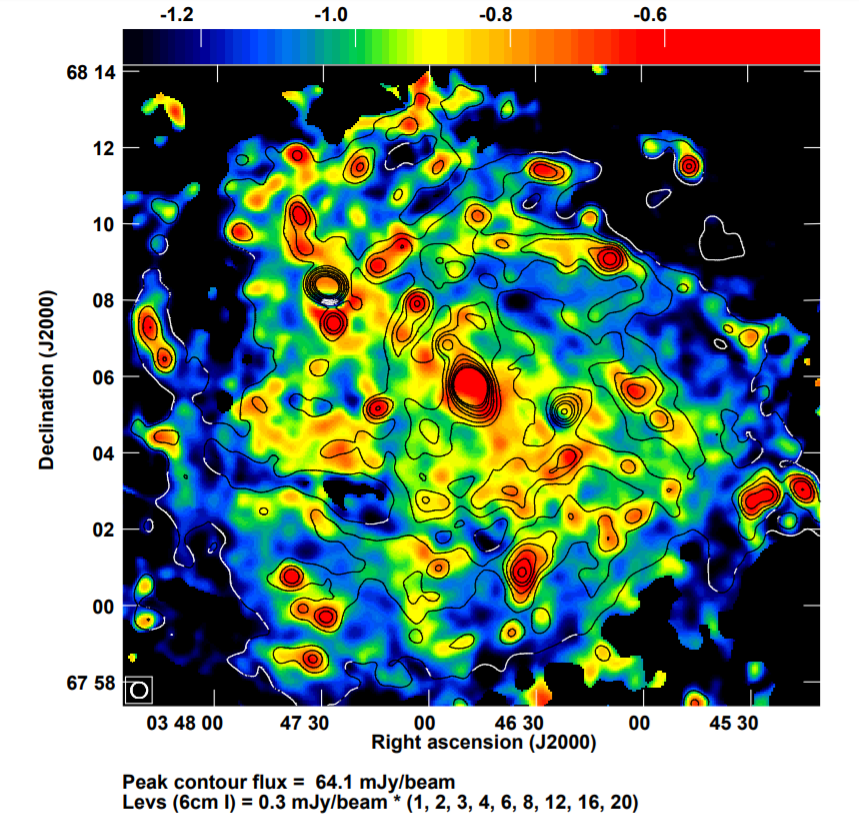
\includegraphics[scale = 0.45]{icspectral.png}
\caption{This is the spectral index map obtained between $\lambda$6.2~cm and $\lambda$20.1~cm at 25" resolution. Contours show the total intensity at $\lambda$6.2 cm. It has been taken from \citet{2015A&A...578A..93B}.}
\label{specic}
\end{figure}

\subsection{NGC\,628}

\noindent The spectral index map of NGC\,628 can be seen in the Figure \ref{ngc_spectr}. The regions with flatter spectral index values are depicted in red. One can trace the presence of spiral arms in the red regions, and the outer edges of the galaxy have a steeper spectrum, sa shown by the green regions. This shows that the spiral arms have flatter spectral index which are the regions with younger recently formed stars. The steepness in the outer regions is indicative of the older electron population, where the flux density of the LOFAR map is much higher than that of the VLA map.\\

In order to study the star forming regions in NGC\,628, and understand the flattening of the various regions, we overlay an H alpha image onto the spectral index map\footnote{H-alpha emission has a wavelength of 656.28 nm in the visible spectral range. It occurs when a hydrogen electron falls from its third to second lowest energy level.}. We can see a clear correlation between the flattening of the spectrum and the H alpha region. We can also see the two arms of the galaxy that are traced by both the H alpha region and the flatter (depicted by red) in the galaxy. The steeper part of the galaxy that contains the synchrotron emission from the diffuse electrons can be seen between the two arms. This shows that most of the star formation takes place in the arms while the diffuse older electrons that have traveled away from the spiral arms are present in the inter-arm regions. This part of the galaxy is marked as region \textbf{A} ,\textbf{B} and region \textbf{E} in the Figure \ref{hlaph_ng}.\\
\begin{figure}
\centering
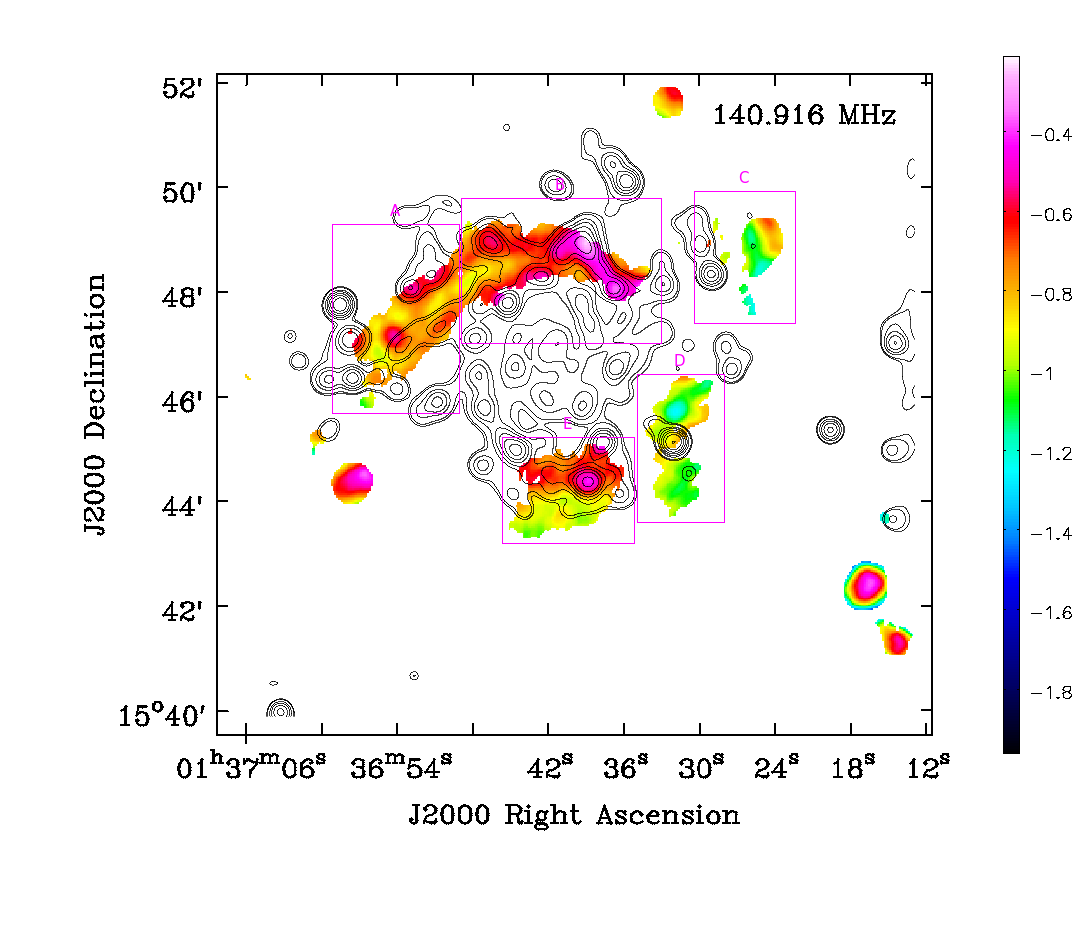
\includegraphics[scale = 0.4]{h-alpha_regions.png}
\caption{This image depicts the correlation of the flatter spectral index and the presence of H-$\alpha$ emission. The contours are 0.5, 1, 3, 5, 8, 12, 18, 32, 44, 80 of the h-alpha map with unit contour level of 5~mJy/beam. The regions are described in the text.}
\label{hlaph_ng}
\end{figure}
However, something peculiar is seen in the region marked as \textbf{D}. It appears to be much steeper even though there is a clear increase of the intensity in the H alpha map. In order to understand it better, I overlay the LOFAR map with an optical image as can be seen in the Figure \ref{optical}. In this image, this region is shown in yellow meaning that it is not an H II region. However, in the paper \citet{1980ApJ...241..573K}, this source has been listed as an H II region, of the name ``NGC 0628:[H76] 566", although not much is known about this region. Hence, this discrepancy may be because the red continuum has not been sufficiently subtracted in the H alpha map, which may be because of the presence of a bright star in H alpha image. \\
\begin{figure}
\centering
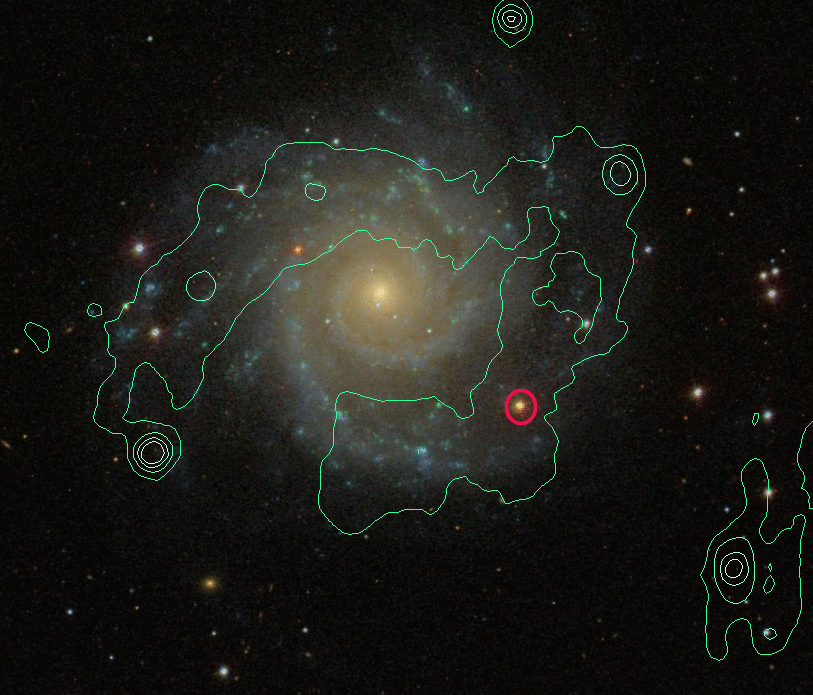
\includegraphics[scale = 0.3]{ngc_optical_edit.png}
\caption{Overlaying the LOFAR map onto an optical image from SDSS shows that this region contains a stellar object. This was done inorder to understand the region marked \textbf{D}.}
\label{optical}
\end{figure}
The Figure \ref{spectr} shows the various regions and their correlations. The two spiral arms have different slopes in the correlation plot. This may be because of different levels of star formation in the two arms, which gives rise to different levels of thermal absorption in the galaxy at various regions. It is interesting to note that the Figure \ref{corr_ic}, depicting the same correlations does not show this feature of differing slopes.
\begin{figure}
	%\centering
	\subfloat[]{{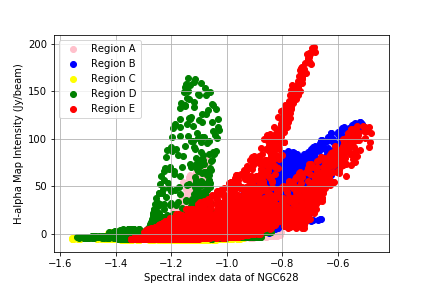
\includegraphics[scale = 0.62]{13Regions_halpha.png}}}
	\centering
	\subfloat[]{{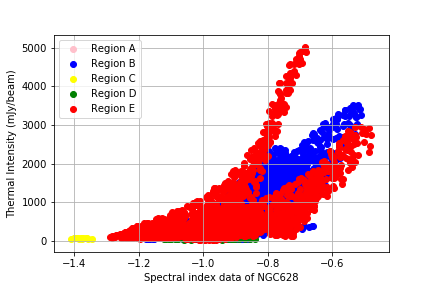
\includegraphics[scale = 0.62]{13Regions_thermal_region_all.png}}}
	\caption{Correlation plots of the thermal intensity values value with the spectral index map values, for each pixel. The various regions have different slops of correlation, which is interesting. \textit{Left:} The correlation plot of the H-alpha map flux density. the region marked \textbf{D} in this case seems to have a higher flux in H-alpha map, but with a steep spectral index. \textit{Right:} The correlation plot of the thermal radio map. The region \textbf{D} in this plot vanishes. Hence, the discrepancy seen in region \textbf{D} was because of an improper continuum subtraction.}
\label{spectr}
\end{figure}


In order to understand the discrepancy in the region \textbf{D}, we try to do the correlation plot using the thermal radio map obtained at a frequency of 3~GHz \citep{2017A&A...600A...6M}. In this case, the region \textbf{D} does not have a higher intensity value in the thermal map, and hence, the steep spectral index is correct. This map can be seen in the Figure \ref{ngc_ther}. 

\begin{figure}
\centering
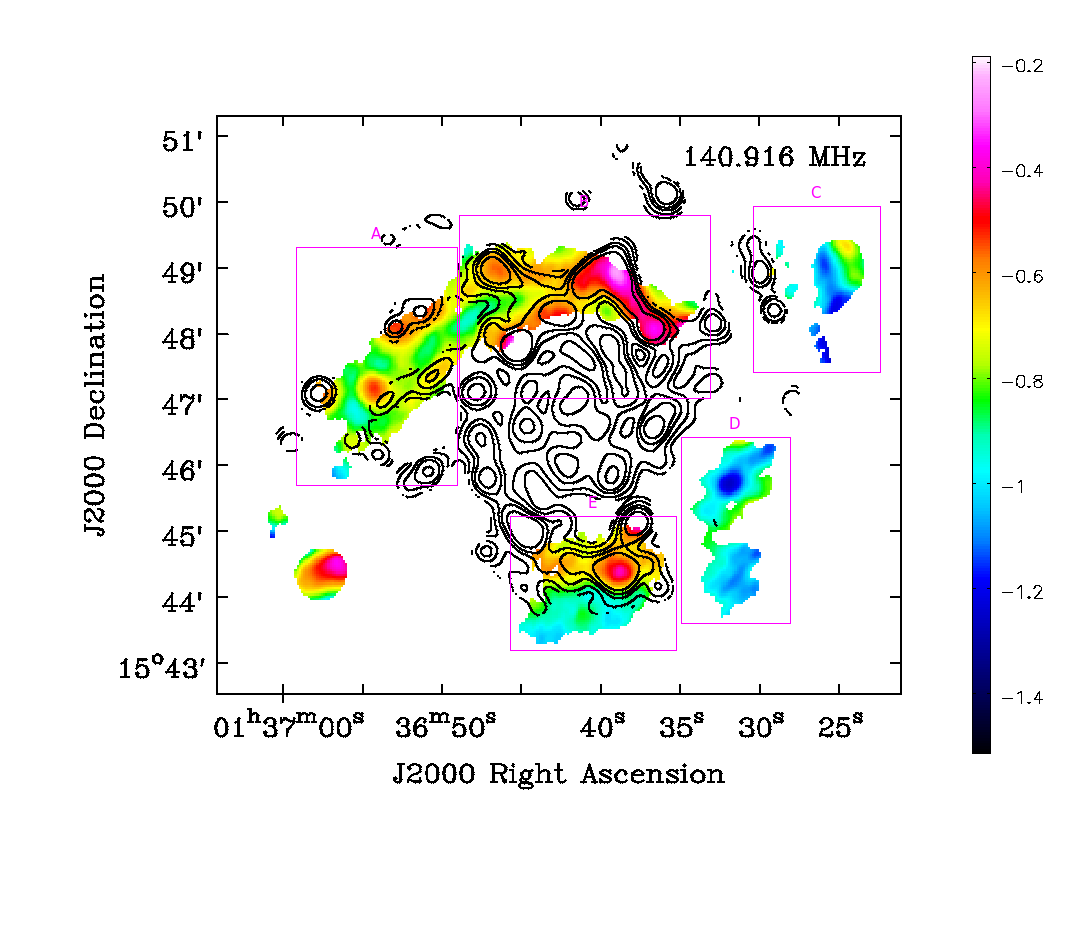
\includegraphics[scale = 0.5]{ngc_ther.png}
\caption{Correlation of the flatter spectral index in NGC\,628 and the presence of thermal radio emission at 3~GHz frequency. The contours are 0.1, 0.2, 0.4, 0.6, 1 $\times$ 0.1~mJy/beam.}
\label{ngc_ther}
\end{figure}



\paragraph{Integrated flux density:} The integrated flux density values for NGC\,628 for successive radii in rings with a width of 0.5' (about 1.1~kpc) are obtained, with the center of the rings aligned at the center of the galaxy. The plot with the radial profile using the obtained values is shown in Figure \ref{ngc_ring}. This is done for the images of the two frequencies- 145~MHz and 3~GHz. I then find the integrated flux density of the galaxy up to a radius of 5' of NGC\,628 (around 11~kpc) in the VLA map at a frequency of 3~GHz to be 108 $\pm$ 3~mJy. The value for the LOFAR map for this integrated flux at 145~MHz is 680 $\pm$ 120~mJy. This value seems to show that the spectral index of the map is -0.61. This shows that overall, synchrotron emission dominates in the LOFAR frequency for the galaxy. 

\begin{figure}
\centering
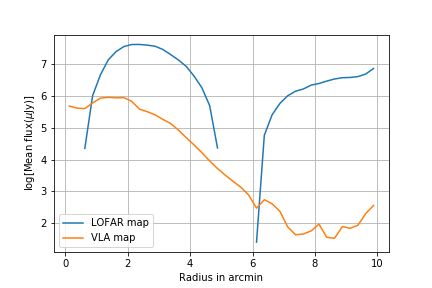
\includegraphics[scale = 0.7]{LOFAR_VLA_ring.png}
\caption{The radial profile of the galaxy NGC\,628 i.e., radius vs log of integrated flux density for 3~GHz map \citep{2017A&A...600A...6M} and 145~MHz LOFAR map.}
\label{ngc_ring}
\end{figure}

\section{Star Formation in the two galaxies}
In this section, I shall discuss star formation in the two galaxies- IC\,342 and NGC\,628. Star formation in spiral galaxies is usually seen to take place in the spiral arms. It would be interesting to understand whether spiral arms trigger star formation, or if they rearrange the stars and molecular gas such that majority of star formation (SF) is seen in the arms. One may hypothesize that the sudden increase in the density in the spiral arms results in mechanisms of gravitational collapse such that conditions for SF is acquired. Stars are formed from molecular gas. However, most of the molecular H$_2$ is cold (10-20~K) and hence, invisible. It is also not easily excitable as requires a large amount of energy to be excited\footnote{First level rotational level, which is accessible only from a quadrupolar transaction, occurs at a temperature above 500~K.}. Hence, CO, the next most abundant molecule is used as its tracer. Using the well known Kennicutt-Schmidt (K-S) law, one can obtain the SF Rate (SFR) of a galaxy \citep{1959ApJ...129..243S}:
\begin{equation}
\Sigma_{SFR} \textrm{(M}_\odot\textrm{ yr}^{-1} \textrm{kpc}^{-2}) \propto (\Sigma_{gas})^N \textrm{(M}_\odot \textrm{kpc}^{−2})
\end{equation}
Here, $\Sigma_{SFR}$ represents the  SFR surface density and $\Sigma_{gas}$ represents the gas surface density. Usually, the gas surface density is replaced by the H$_2$ as most of the molecular gas is in this form. Then with the help of the CO surface density, using a conversion factor, one can obtain the $\Sigma_{H_2}$.\\
\noindent In the paper \citet{2014PASJ...66...27P}, it is found that IC\,342 is an H$_2$ dominated spiral galaxy where significant amount of SF could occur. The SF mechanisms discused in the paper include gravitational instability in the disk and at the galactic center, and a combination of gravitational instability and cloud-cloud collission at the galactic center. This is because the `\textit{N}' value varies from 1.4 in the low-H$_2$ domain (where $\Sigma_{H_2} <<$ 100~M$_{\odot}$ pc$^{-2}$) to 2-3 in the high H$_2$ domain. In the Figure\ \ref{sfric342}, one can see the SFRs obtained from this method, and how it change radially. 


\begin{figure}
  \centering
    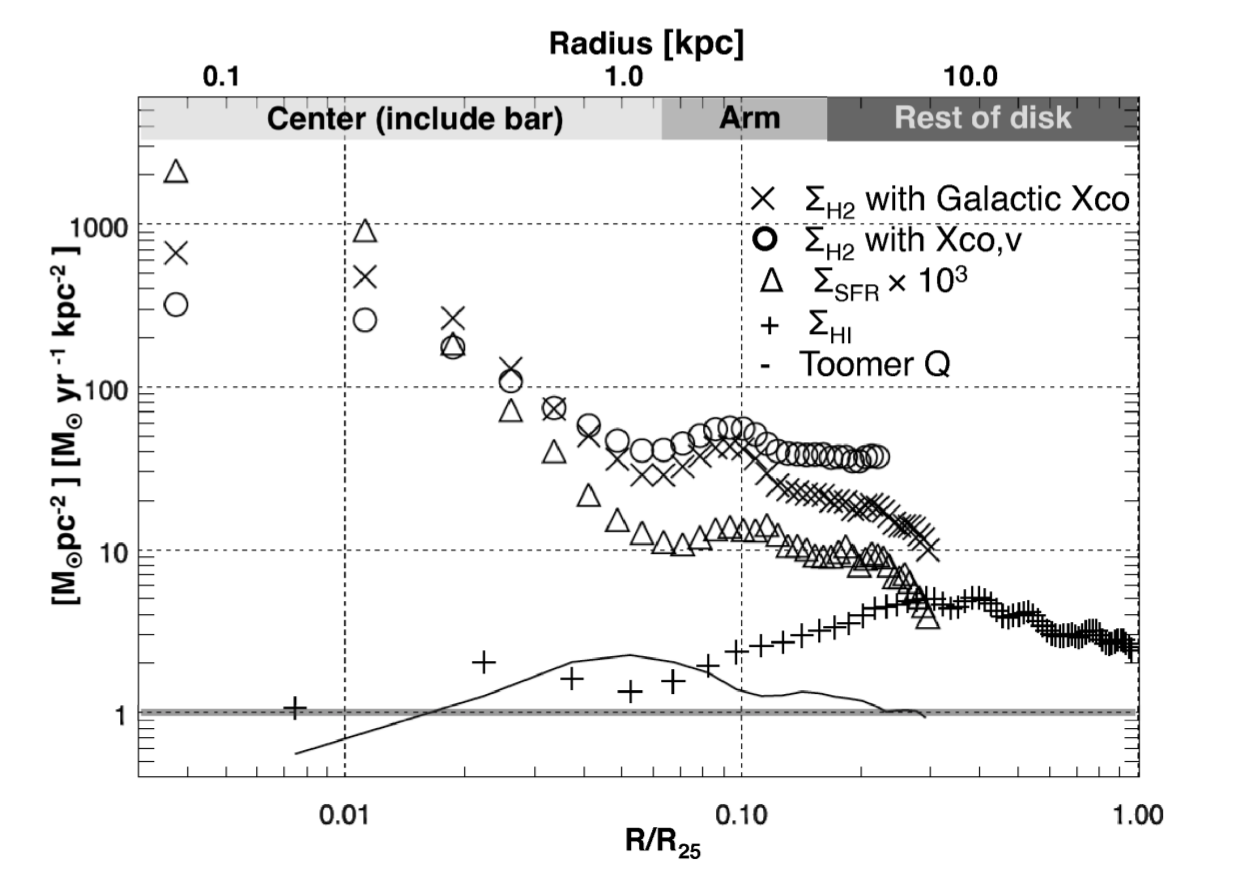
\includegraphics[scale=0.3]{SFRic.png}
  \caption{The SFR are shown as small triangles \citep{2014PASJ...66...27P}. Each radial step here is 10". One can see a similarity in the two plots. In the center, high star formation exists, and that region has a flat spectral index.}\label{sfric342}
\end{figure}

Unfortunately, in NGC\,628, I cannot do a comparison of the spectral indices and the star formation rates, as the flux density at the center of the galaxy is zero. In the paper \citet{2017A&A...600A...6M}, it is seen that NGC\,628 at 8.35~GHz has an asymmetric pattern with a lot of emission coming in from the northern part of the galaxy, and not at the center. This would be in concurrence with the explanation that there is a rapid decline in the star formation at the inner region as described in \citet{2001ApJS..132..129M}. In the JVLA image, at the frequency of 3.1~GHz, there was a presence of `holes' which line up with the type 1 H I holes\footnote{HI holes are characterized by the absence of neutral hydrogen and have the dimensions from 100~pc to 1~kpc.}, as seen in \citet{2011AJ....141...23B}. The absence of flux density can be attributed to rapid decline in SFR. However, I cannot be ascertain this in any way.

Using the Star Formation Rates given in \citet{2011PASP..123.1347K}, we can try to understand why the median values of the spectral indices of the two galaxies are so different. The SFR of IC\,342 is 1.87~M$_{\odot}$ pc$^{-1}$ while that of NGC\,628 is 0.68~M$_{\odot}$ pc$^{-1}$. Thus one could expect a flatter spectral index of IC\,342 than that in NGC\,628. Also, IC\,342 suffers from a higher level of thermal absorption, indicating the presence of a higher level of star formation, especially at the nucleus of the galaxy.

\section{Discussion}
Further work needs to be done to fully understand the significance of thermal absorption in the galaxies at such low frequencies. Measurement of the spectra at low frequencies should be done using the LOFAR LBA data, and obtain the spectral energy distribution to see how much flux density of the galaxies is removed due to thermal absorption. 

\end{document}
